%\subsection{Neocortical Layer 4/5 Pyramidal Cell Test Suite}
\subsubsection{Performance of Layer 5 Prefrontal cortex Pyramidal Neuron on NeuronUnit tests of model data agreement}
\cite{van2016bluepyopt}
A suite of neuronunit tests containing the tests: rheobase value, membrane voltage time constant ($tau_{m})$, input resistance was computed. This multi-compartment, conductance based model served as a useful benchmark, for us to evaluate the relative performance of reduced model fits.

Significant development work went into making the model eligible to take NeuronUnit tests, by way of creating a specially dedicated NeuronUnit backend, to run this complicated conductance based multi-compartment model originating from the blue brain model \cite{markram2015reconstruction}.

This elaborate biophysical model includes the backpropogating dendritic action potential.
\url{}



\begin{figure}
\begin{center}


\centering
\begin{subfigure}{.2\textwidth}
  \centering
    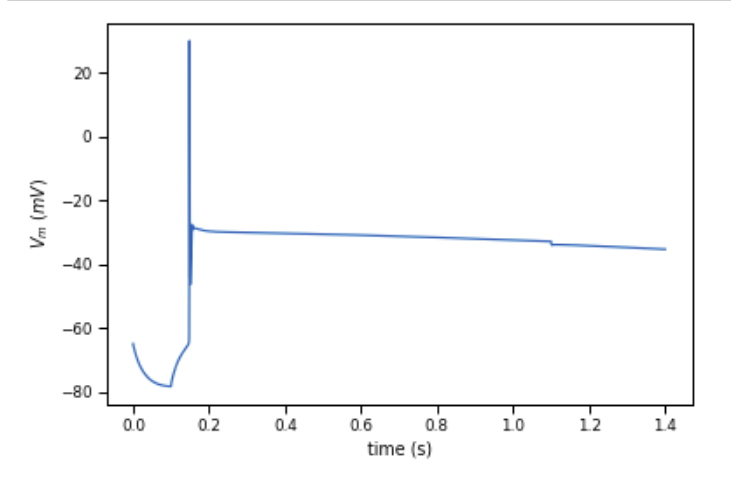
\includegraphics[scale=0.5]{figures/correct_active_l5pc.png}
    \caption{A current injection sufficient for causing a single spike is applied for a whole second from $100ms-1100ms$}
  \label{fig:sub1}
\end{subfigure}

\centering
\begin{subfigure}{.2\textwidth}
  \centering
    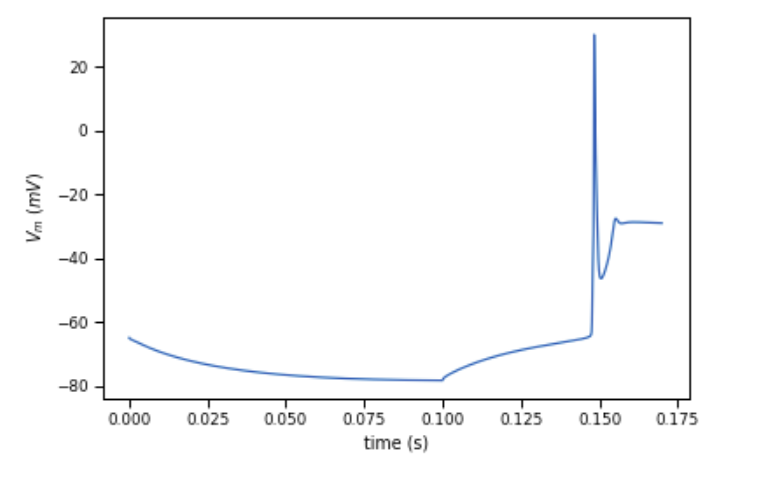
\includegraphics[scale=0.5]{figures/spike_shape.png}
    \caption{The spike shape is very brief in duration, and so it is worth zooming in for a closer look}
  \label{fig:sub1}
\end{subfigure}


\begin{subfigure}{.2\textwidth}
  \centering
    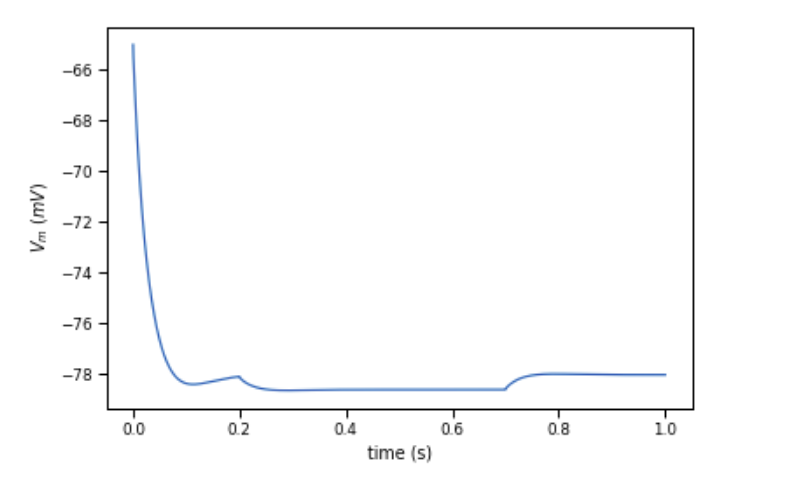
\includegraphics[scale=0.5]{figures/correct_passive_l5pc.png}
    \caption{A current injection value of -$10pA$ is applied to the cell for the duration of $200ms-700ms$}
  \label{fig:sub2}
\end{subfigure}
\label{fig:test}
\end{center}
\end{figure}


A test suite was constructed using NeuroElectro for the layer 4/5 Prefrontal Cortex pyramidal cell, and we were able to evaluate this layer 5 PC cells against the criteria of the neuroelectro test suite. 

\begin{table}[ht]
\centering
\resizebox{\textwidth}{!}{
\begin{tabular}{llll}
\toprule
{} & observations &   predictions & Z-Scores \\
\midrule
RheobaseTest                   &    213.85 pA &      225.0 pA &  0.06542 \\
InputResistanceTest            &  120.67 Mohm &  50.7 megaohm &  -0.9013 \\
TimeConstantTest               &     15.73 ms &      16.76 ms &   0.1409 \\
CapacitanceTest                &    150.58 pF &     330.66 pF &    1.289 \\
RestingPotentialTest           &    -68.25 mV &     -78.04 mV &   -1.499 \\
InjectedCurrentAPWidthTest     &      1.21 ms &       0.15 ms &   -1.979 \\
InjectedCurrentAPAmplitudeTest &     80.44 mV &      89.58 mV &   0.7174 \\
InjectedCurrentAPThresholdTest &    -42.74 mV &     -59.57 mV &   -2.094 \\
\bottomrule
\end{tabular}}
\end{table}
The corresponding statistics were
$(\chi^{2},p_{value})=(13.5609360364, 0.093951963105254)$

    
It is worth noting that the layer 5 neocortical pyramidal neuron was very slow to dispatch relative to the reduced models developed in this thesis work. Where as a typical reduced model described here evaluated in the order of $~0.0025 seconds$, this model on average took $5.74$, for a single run and $34.8$ to solve for the models Rheobase, current.


This model was pre-optimized to fit to spike times and F/I mainly, and so it should not necassarily be expected to fit other electrical charactersistics of the cell. Only the rheobase test, and the time constant test seemed to fall within the range of biological plausibility.
None the less, this model remains a useful benchmark for reduced neuronal models.